\chapter{Экспериментальная часть}

В данном разделе описаны замерные эксперименты и представлены результаты исследования.

\section{Технические характеристики}
Технические характеристики устройства, на котором выполнялось исследование \cite{bib:5}:
\begin{itemize}
	\item 8 ГБ оперативной памяти;
	\item процессор Apple M2 (тактовая частота~---~до $3.5$ГГц);
    \item операционная система macOS Ventura 13.0.
\end{itemize}

\section{Измерение процессорного времени выполнения реализаций алгоритмов}

Для измерения процессорного времени выполнения реализаций алгоритмов была использована функция языка $C$~---~$clock\_gettime$, которая позволяет получить текущее процессорное время в наносекундах \cite{bib:6}.

\subsection{Худший случай}

В таблице \ref{table:time_worst} представлены результаты измерений процессорного времени выполнения в зависимости от размера массива для худших случаев алгоритмов сортировок. На рисунке \ref{img:time_worst} представлена зависимость времени выполнения от длины массива.

\begin{table}[h]
  \caption{\label{table:time_worst} Результаты замеров процессорного времени для худшего случая (в нс)}
  \begin{center}
    \begin{tabular}{|r|r|r|r|}
      \hline
      Длина массива & Блочная & Пирамидальная & Подсчетом\\ \hline
1000 & 806800 & 460230 & 849980 \\ \hline 
2000 & 1474230 & 1022930 & 840620 \\ \hline 
3000 & 2153590 & 1680120 & 894170 \\ \hline 
4000 & 2894810 & 2230680 & 816990 \\ \hline 
5000 & 3636540 & 2893940 & 880270 \\ \hline 
6000 & 4500900 & 3568040 & 835930 \\ \hline 
7000 & 5038730 & 4188360 & 840940 \\ \hline 
8000 & 5761830 & 4856270 & 846700 \\ \hline 
9000 & 6441740 & 5500050 & 847050 \\ \hline 
10000 & 7223430 & 6159050 & 850000 \\ \hline 


    \end{tabular}
  \end{center}
\end{table}

\newpage

\noindent
\begin{figure}[h!]
	\centering
    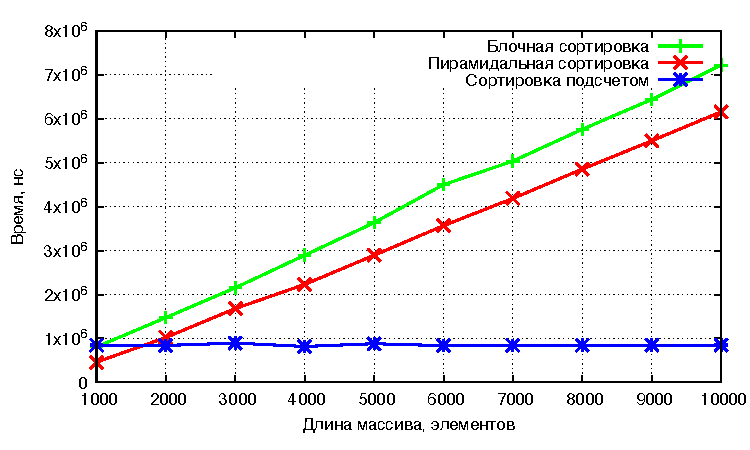
\includegraphics[width=0.75\linewidth]{../data/time_worst}
    \caption{Результаты замеров времени для худшего случая}
    \label{img:time_worst}
\end{figure}


\subsection{Лучший случай}

В таблице \ref{table:time_best} представлены результаты измерений процессорного времени выполнения в зависимости от размера массива для лучших случаев алгоритмов сортировок. На рисунке \ref{img:time_best} представлена зависимость времени выполнения от длины массива.

\begin{table}[h]
  \caption{\label{table:time_best} Результаты замеров процессорного времени для лучшего случая (в нс)}
  \begin{center}
    \begin{tabular}{|r|r|r|r|}
      \hline
      Длина массива & Блочная & Пирамидальная & Подсчетом\\ \hline
1000 & 178780 & 98770 & 13360 \\ \hline 
2000 & 244380 & 148500 & 10950 \\ \hline 
3000 & 302290 & 203300 & 15100 \\ \hline 
4000 & 400050 & 272240 & 18780 \\ \hline 
5000 & 497950 & 339660 & 25180 \\ \hline 
6000 & 616370 & 406350 & 26280 \\ \hline 
7000 & 705840 & 478020 & 33700 \\ \hline 
8000 & 792700 & 547480 & 35440 \\ \hline 
9000 & 904100 & 624620 & 42700 \\ \hline 
10000 & 997280 & 677370 & 47740 \\ \hline 



    \end{tabular}
  \end{center}
\end{table}

\newpage

\noindent
\begin{figure}[h!]
	\centering
    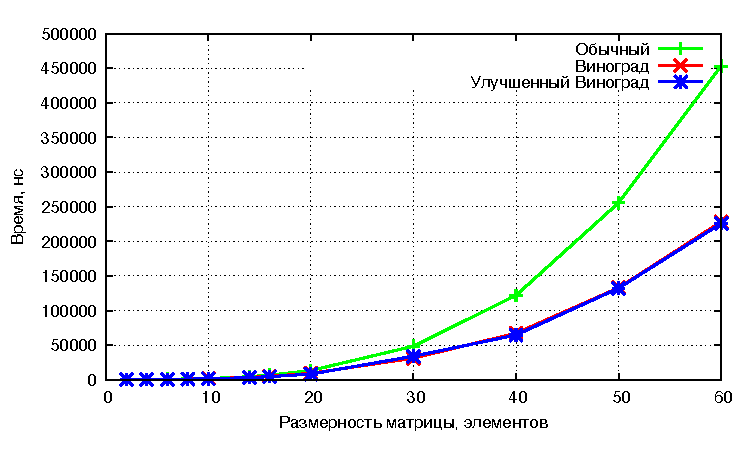
\includegraphics[width=0.75\linewidth]{../data/time_best}
    \caption{Результаты замеров времени для лучшего случая}
    \label{img:time_best}
\end{figure}

\subsection{Случайный случай}

В таблице \ref{table:time_random} представлены результаты измерений процессорного времени выполнения в зависимости от размера массива для алгоритмов сортировок на случайных входных данных. На рисунке \ref{img:time_random} представлена зависимость времени выполнения от длины массива.

\begin{table}[h]
  \caption{\label{table:time_random} Результаты замеров процессорного времени для случайного случая (в нс)}
  \begin{center}
    \begin{tabular}{|r|r|r|r|}
      \hline
      Длина массива & Блочная & Пирамидальная & Подсчетом\\ \hline
1000 & 499350 & 468690 & 20330 \\ \hline 
2000 & 1033070 & 1009490 & 22670 \\ \hline 
3000 & 1590200 & 1624070 & 29670 \\ \hline 
4000 & 2097670 & 2211810 & 40560 \\ \hline 
5000 & 2614480 & 2901950 & 48720 \\ \hline 
6000 & 3104580 & 3470970 & 55820 \\ \hline 
7000 & 3487130 & 4106930 & 59860 \\ \hline 
8000 & 3945090 & 4754490 & 66900 \\ \hline 
9000 & 4358250 & 5430200 & 69750 \\ \hline 
10000 & 4769100 & 6104990 & 74730 \\ \hline 


    \end{tabular}
  \end{center}
\end{table}

\newpage

\noindent
\begin{figure}[h!]
	\centering
    \includegraphics[width=0.75\linewidth]{../data/time_random}
    \caption{Результаты замеров времени для случайного случая}
    \label{img:time_random}
\end{figure}

\section{Измерение объёма потребляемой памяти реализаций алгоритмов}

В таблице \ref{table:memory} представлены результаты измерения потребляемой памяти в зависимости от длины массива. На рисунке \ref{img:memory} представлена зависимость потребляемой памяти от длины массива.

\begin{table}[h]
  \caption{\label{table:memory} Результаты замеров потребляемой памяти (в байтах)}
  \begin{center}
    \begin{tabular}{|r|r|r|r|}
      \hline
      Длина массива & Блочная & Пирамидальная & Подсчетом\\ \hline
1000 & 24336 & 8056 & 32136 \\ \hline 
2000 & 48336 & 16056 & 56136 \\ \hline 
3000 & 72336 & 24056 & 80144 \\ \hline 
4000 & 96336 & 32056 & 104144 \\ \hline 
5000 & 120336 & 40056 & 128144 \\ \hline 
6000 & 144336 & 48056 & 152144 \\ \hline 
7000 & 168336 & 56056 & 176144 \\ \hline 
8000 & 192336 & 64056 & 200144 \\ \hline 
9000 & 216336 & 72056 & 224144 \\ \hline 
10000 & 240336 & 80056 & 248144 \\ \hline 

    \end{tabular}
  \end{center}
\end{table}

\noindent
\begin{figure}[h!]
	\centering
    \includegraphics[width=0.7\linewidth]{../data/memory.pdf}
    \caption{Результаты замеров памяти}
    \label{img:memory}
\end{figure}

\newpage